\documentclass[english,a4paper,12pt]{article}
\usepackage[utf8]{inputenc} %for å bruke æøå
\usepackage{babel}
\usepackage{verbatim} %for å inkludere filer med tegn LaTeX ikke liker
\usepackage[document]{ragged2e}
\bibliographystyle{plain}
\usepackage{amsmath}
\usepackage{ulem}
\usepackage[pdftex]{graphicx}
\usepackage{gensymb}
\usepackage{float}
\usepackage{hyperref}
\usepackage{amssymb}
\usepackage[top=0.6in, bottom=0.8in, left=0.9in, right=0.7in]{geometry}
\usepackage{listings}
\usepackage{color}
\usepackage{tikz}

\usepackage{filecontents}
\begin{filecontents}{mybib.bib}
@book{Langtangen-2016,
   author    = "Hans Petter Langtangen \& Svein Linge",
   title     = "Finite Difference Computing
with PDEs - A Modern Software
Approach",
   publisher = "Center for Biomedical Computing, Simula Research Laboratory
Department of Informatics, University of Oslo
Department of Process, Energy and Environmental Technology,
University College of Southeast Norway",
   address   = "\url{https://hplgit.github.io/fdm-book/doc/pub/book/pdf/fdm-book-4screen.pdf}",
   pages   = "247--288",
   year      = "2016"
}

@unpublished{Analytical1D-Diffusion,
   title     = "The {D}iffusion {E}quation",
   author = "University of Munster, Institute of Theoretical Physics",
   note   = "\url{http://pauli.uni-muenster.de/tp/fileadmin/lehre/NumMethoden/WS0910/ScriptPDE/Heat.pdf}"
}

\end{filecontents}

\usepackage{natbib}
\usepackage{bibentry}
\nobibliography*

\title{Project 5 - FYS4150/FYS3150}
\author{Shako Farhad \& Simon Millerjord}
\date{\today}

\begin{document}

\definecolor{codegreen}{rgb}{0,0.6,0}
\definecolor{codegray}{rgb}{0.5,0.5,0.5}
\definecolor{codepurple}{rgb}{0.58,0,0.82}
\definecolor{backcolour}{rgb}{0.95,0.95,0.92}
 
\lstdefinestyle{mystyle}{
    backgroundcolor=\color{backcolour},   
    commentstyle=\color{codegreen},
    keywordstyle=\color{magenta},
    numberstyle=\tiny\color{codegray},
    stringstyle=\color{codepurple},
    basicstyle=\footnotesize,
    breakatwhitespace=false,         
    breaklines=true,                 
    captionpos=b,                    
    keepspaces=true,                 
    numbers=left,                    
    numbersep=5pt,                  
    showspaces=false,                
    showstringspaces=false,
    showtabs=false,                  
    tabsize=2
}
 
\lstset{style=mystyle}

\maketitle

\begin{abstract}
Rask forklaring på metoder, resultater og konklusjon. Skal kunne lese abstracten og dermed kunne vite hva raporten handler om.
\end{abstract}

\section*{Introduction}
En forklaring på hva som blir gjort, motivasjon for det og annen forskning eller eksempler på liknende raport/eksperiment.\\ \bigskip

\begin{equation} \label{eq:1D-Diffusion}
 \frac{\partial^2 u(x,t)}{\partial x^2} =\frac{\partial u(x,t)}{\partial t}, t> 0, x\in [0,1]
\end{equation}

\section*{Theoretical models and methods}
We created a program in LabView that read sound signals from a microphone and both wrote those signals to a file in the 'lvm' format. The sound signals from the microphone went through an amplifier and then the DAQ wrote the signals to a file that was stored on the computer. We chose the sampling frequency to be $20000$ Hz because we believed that the highest signal frequency would be at around $8000$ Hz. From the Nyquist-Shannon sampling theorem we knew that we had to select a sampling frequency that was two times the highest signal frequency. And because we wanted to avoid loss of data from inadequate sampling frequency, we added another $4000$ Hz, giving us a total of $20000$ Hz. \bigskip

The experiment was setup as seen in figure \ref{fig:1}. The water flows down from the white tank, through a tube on the table, behind the laptop, and before it flows in to the blue bucket at the bottom right, the microphone picks up the flow sound. The blue bucket is placed on top of a digital flat scale, measuring in grams. The height of the white tank was measured from the water surface to the floor with a digital laser device, and then subtracted that height with the height from the tube end to the floor. (MÅ VITE HVOR MYE TUBE END TIL FLOOR ER FOR HØYED! FARNAZ SKAL VITE DETTE) We were supposed to reach certain Reynold numbers (50, 500 2000 and 4000) by adjusting the height of the white water tank. \bigskip

\begin{figure}[H]
    \centering
    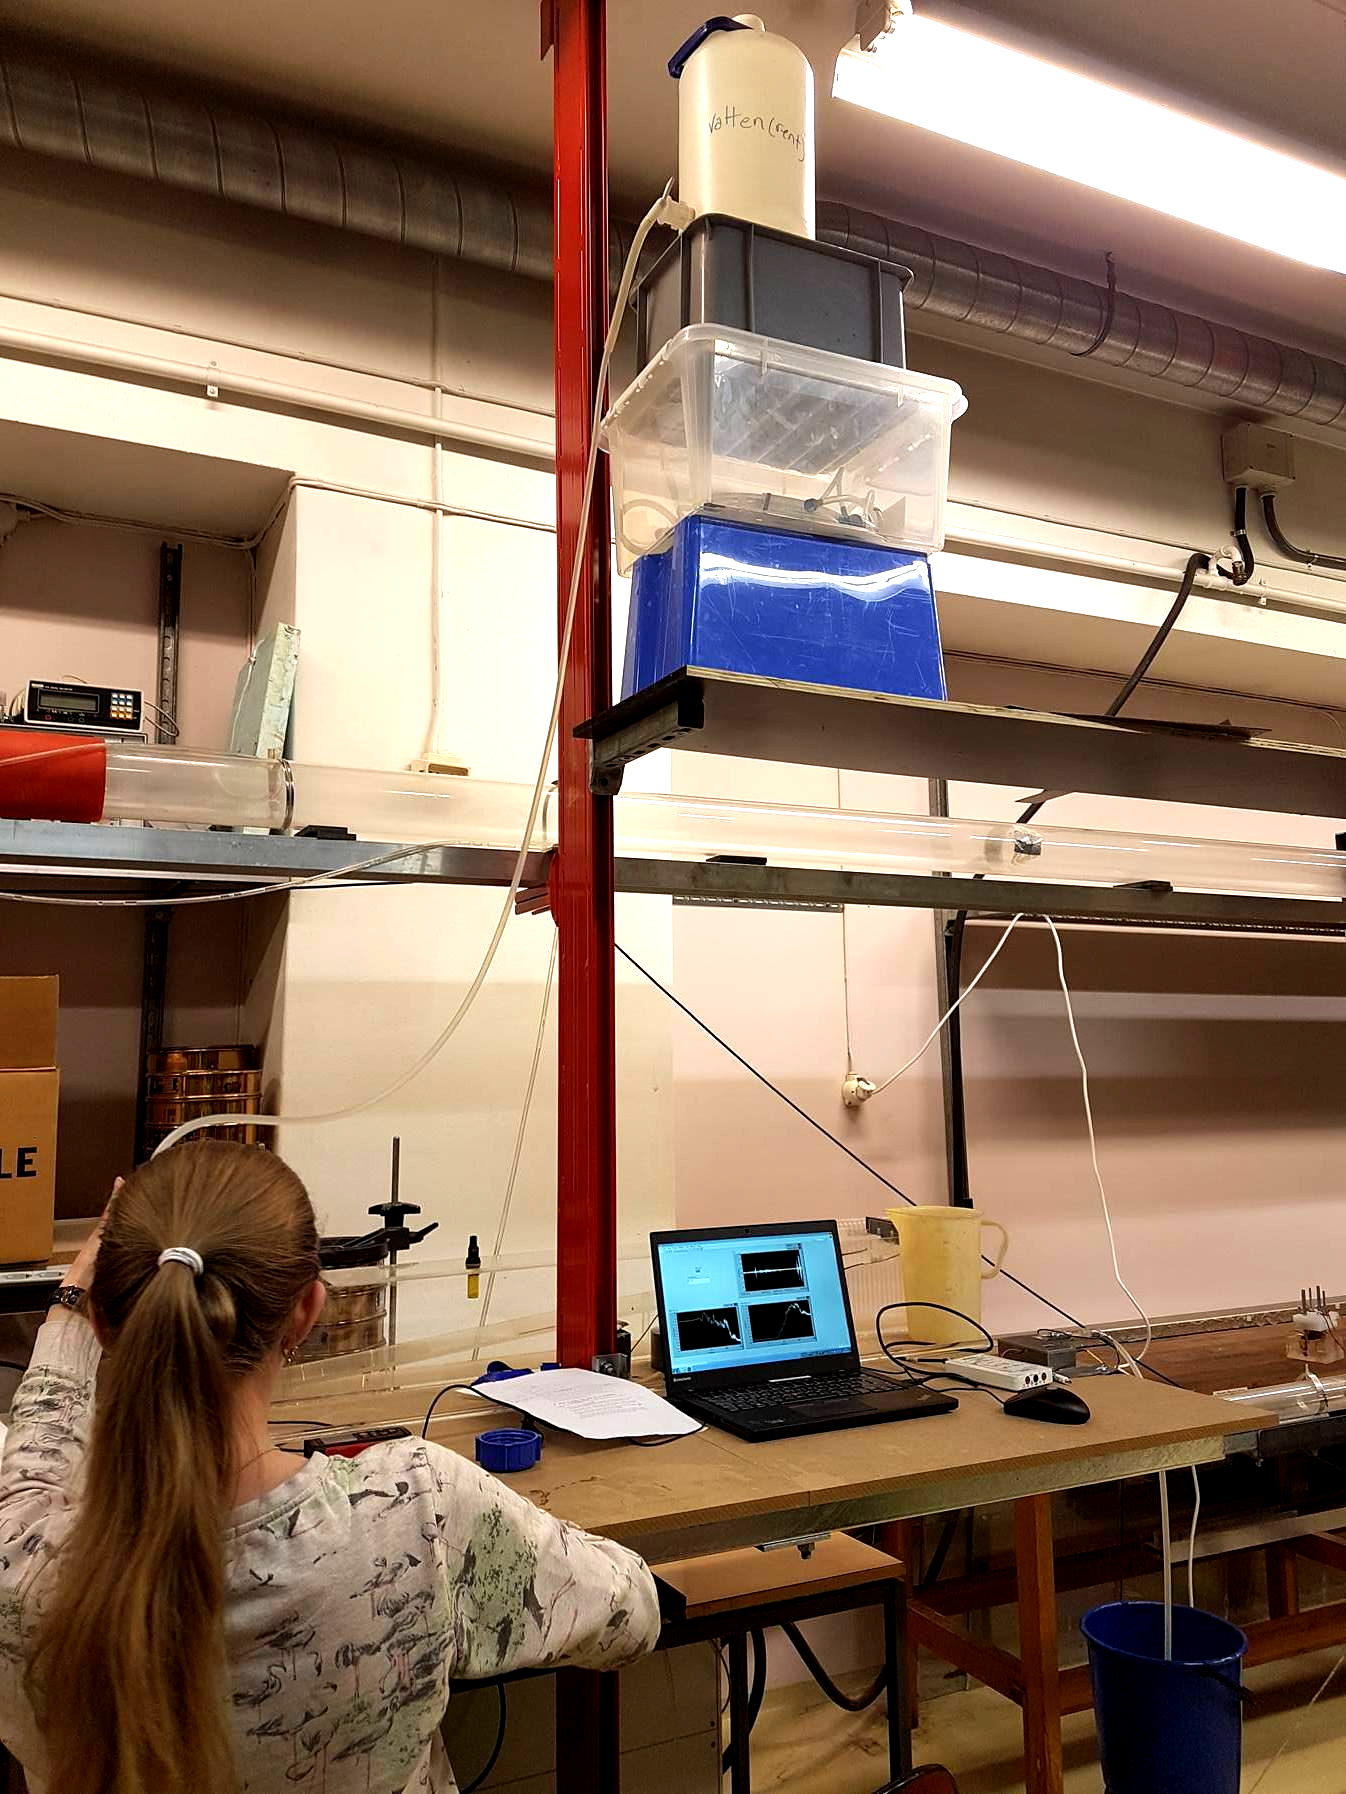
\includegraphics[width=150mm]{ExperimentSetup.png}
    \caption{The setup of the experiments. The white tank at the top contains water that flows through the tube down into the blue bucket. The flow sound signals are measured with a microphone that is amplified and stored on the laptop with the white DAQ box. The water flow was controlled with a valve that was positioned on the table in front of the girl.}
    \label{fig:1}
\end{figure}

The Reynolds number is given by:

$$\text{Re} = \frac{\rho \cdot v \cdot d}{\mu},$$

where $\rho \approx 998.2$ kg/m$^3$ is the water density, $v$ is the water velocity, $d = 0.0079$ m is the inner diameter of the tube, and $\mu = 0.001002 \text{ Pa} \cdot \text{s}$ is the dynamic viscosity. \smallskip

To calculate the velocity, $v$, we used the formula $v=\frac{V}{t\cdot A}$, where $V$ is the volume, $t$ is the time passed, and $A$ is the cross sectional area of the tube. We have $A=\pi \cdot r^2$ and $V=\frac{\text{mass}}{\rho}$. We already knew the mass from the digital scale underneath the blue bucket, and we let the water flow for five minutes every time. In table \ref{tab:1} we can see the calculated values from the different experiments.

\begin{table}[h!]
    \centering
    \begin{tabular}{|c|c|c|c|c|}\hline
    Reynolds number & Velocity [m/s] & Height [m] & Mass [kg] & Time [s] \\ \hline
    52.0075 & 0.0066 & 0.6320 & 0.0970 & 300\\ \hline
    512.0324 & 0.0651 & 0.8440 & 0.9550 & 300\\ \hline
    1940.3614 & 0.2466 & 1.4900 & 3.6190 & 300\\ \hline
    3728.9897 & 0.4738 & 3.1400 & 6.9550 & 300\\ \hline
    \end{tabular}
    \caption{Data from four different experiments where the white tank was placed at different heights.}
    \label{tab:1}
\end{table}

\section*{Results}

\begin{figure}[H]
    \centering
    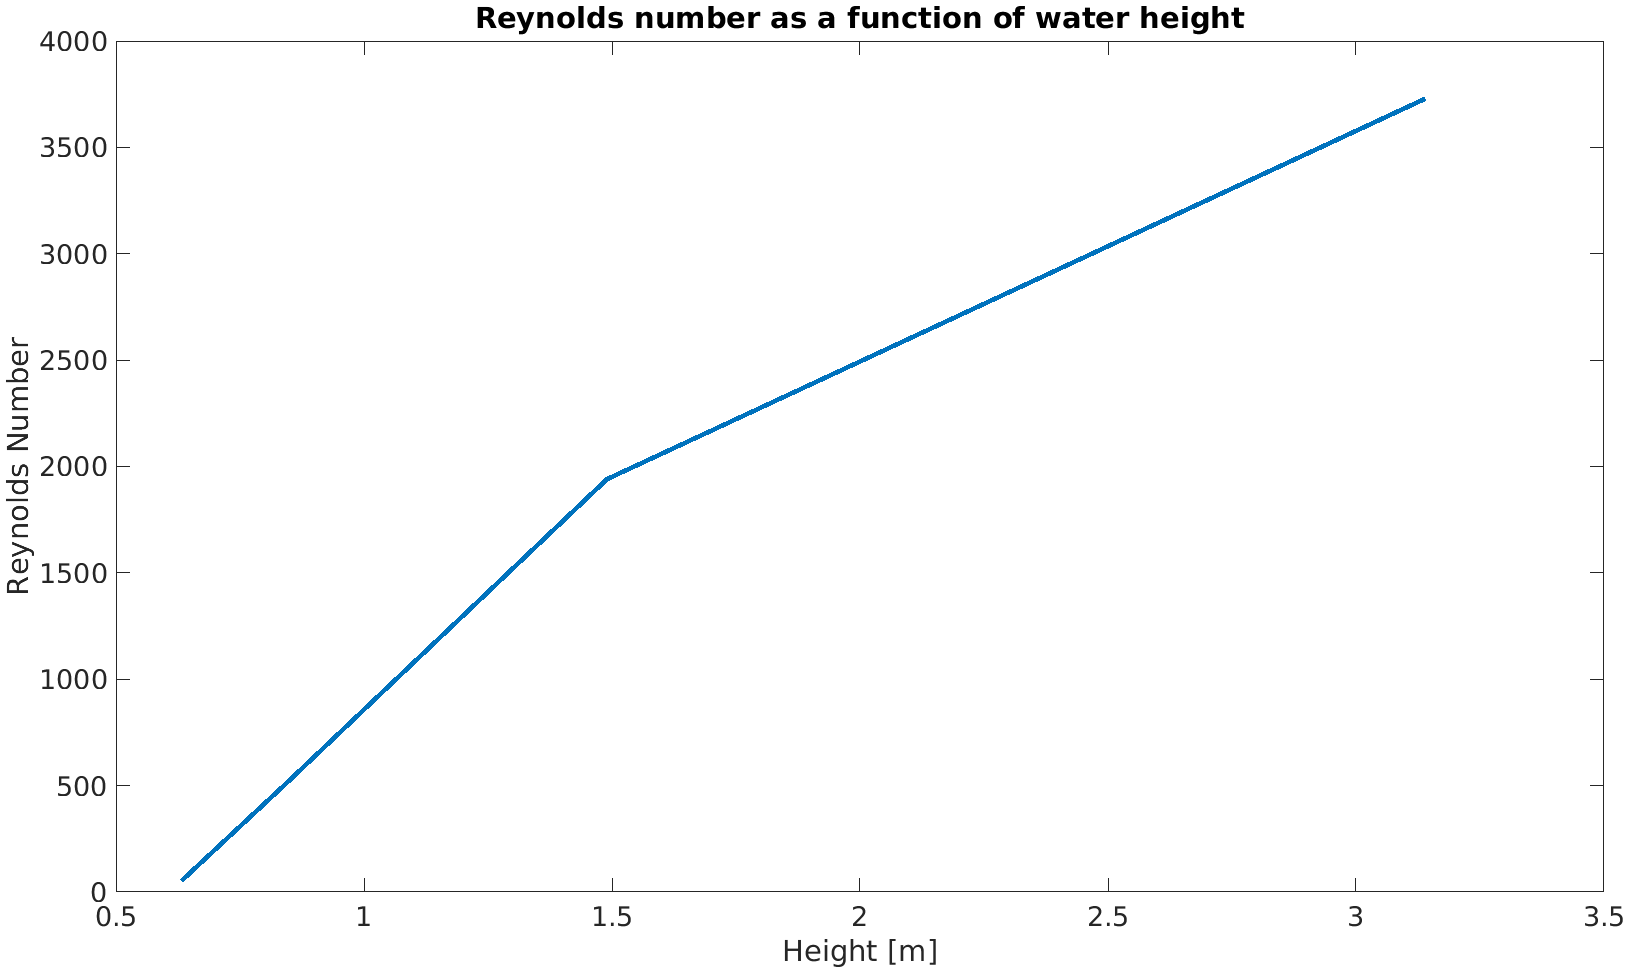
\includegraphics[width=180mm]{ReVsHeightPlot.png}
    \caption{Diminishing returns are starting to be visible already at $1.5$ m height. More data points are needed.}
    \label{fig:2}
\end{figure}

\begin{figure}[H]
    \centering
    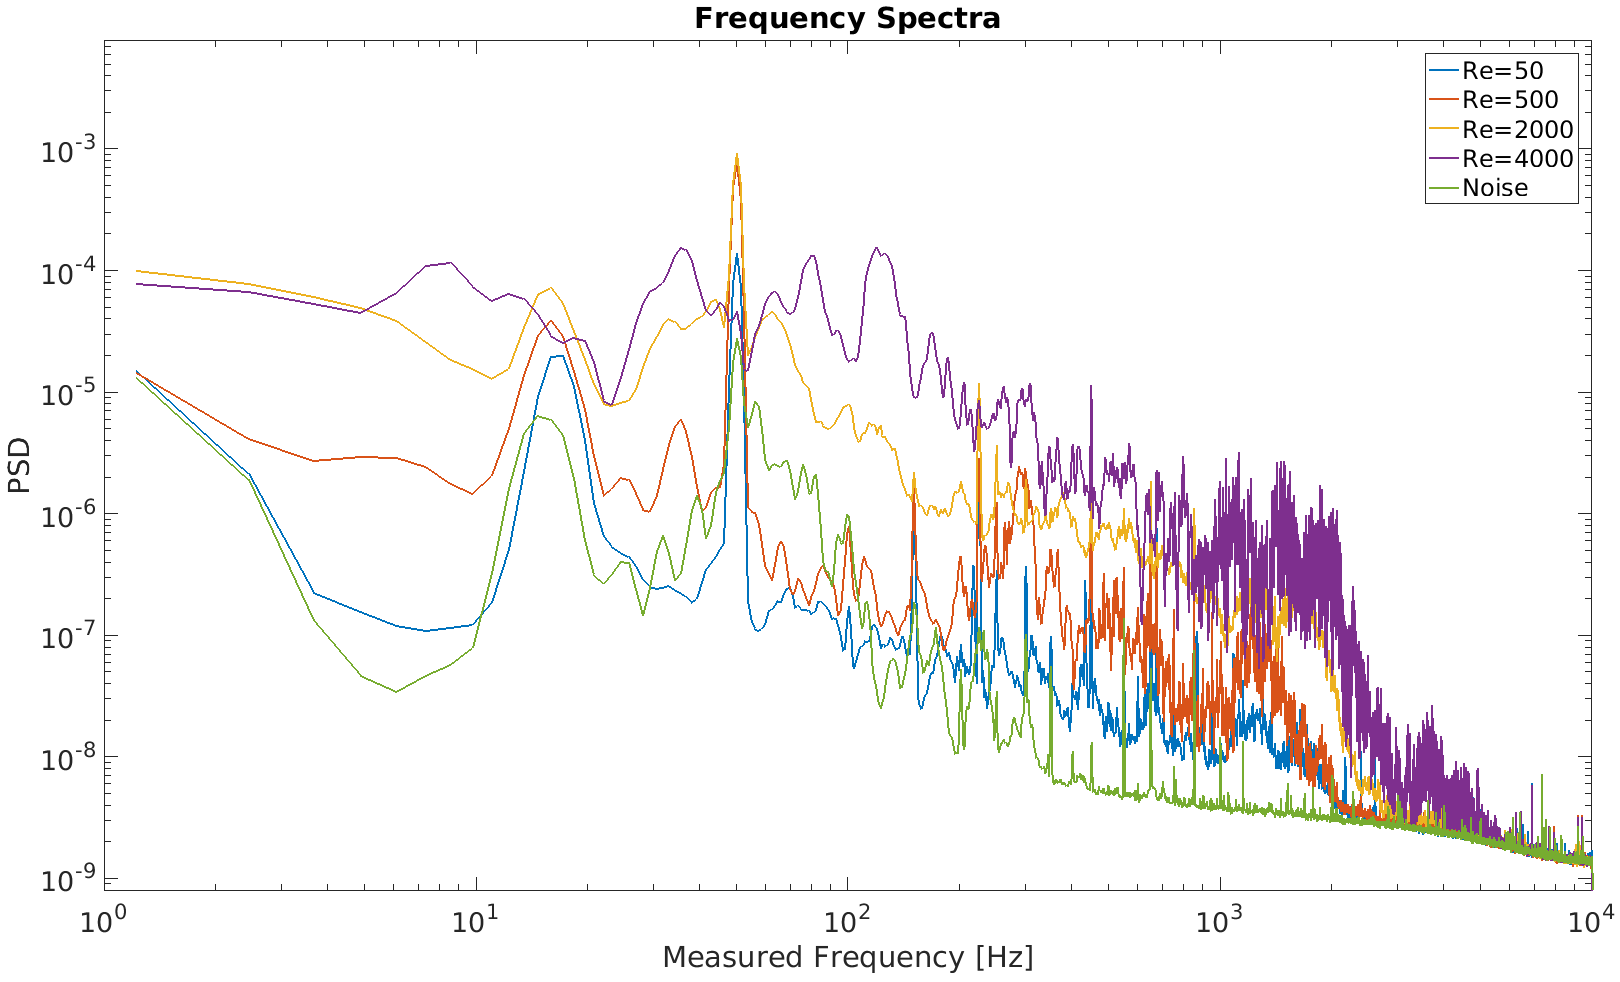
\includegraphics[width=180mm]{FrequencySpectraPlot.png}
    \caption{}
    \label{fig:3}
\end{figure}

\begin{figure}[H]
    \centering
    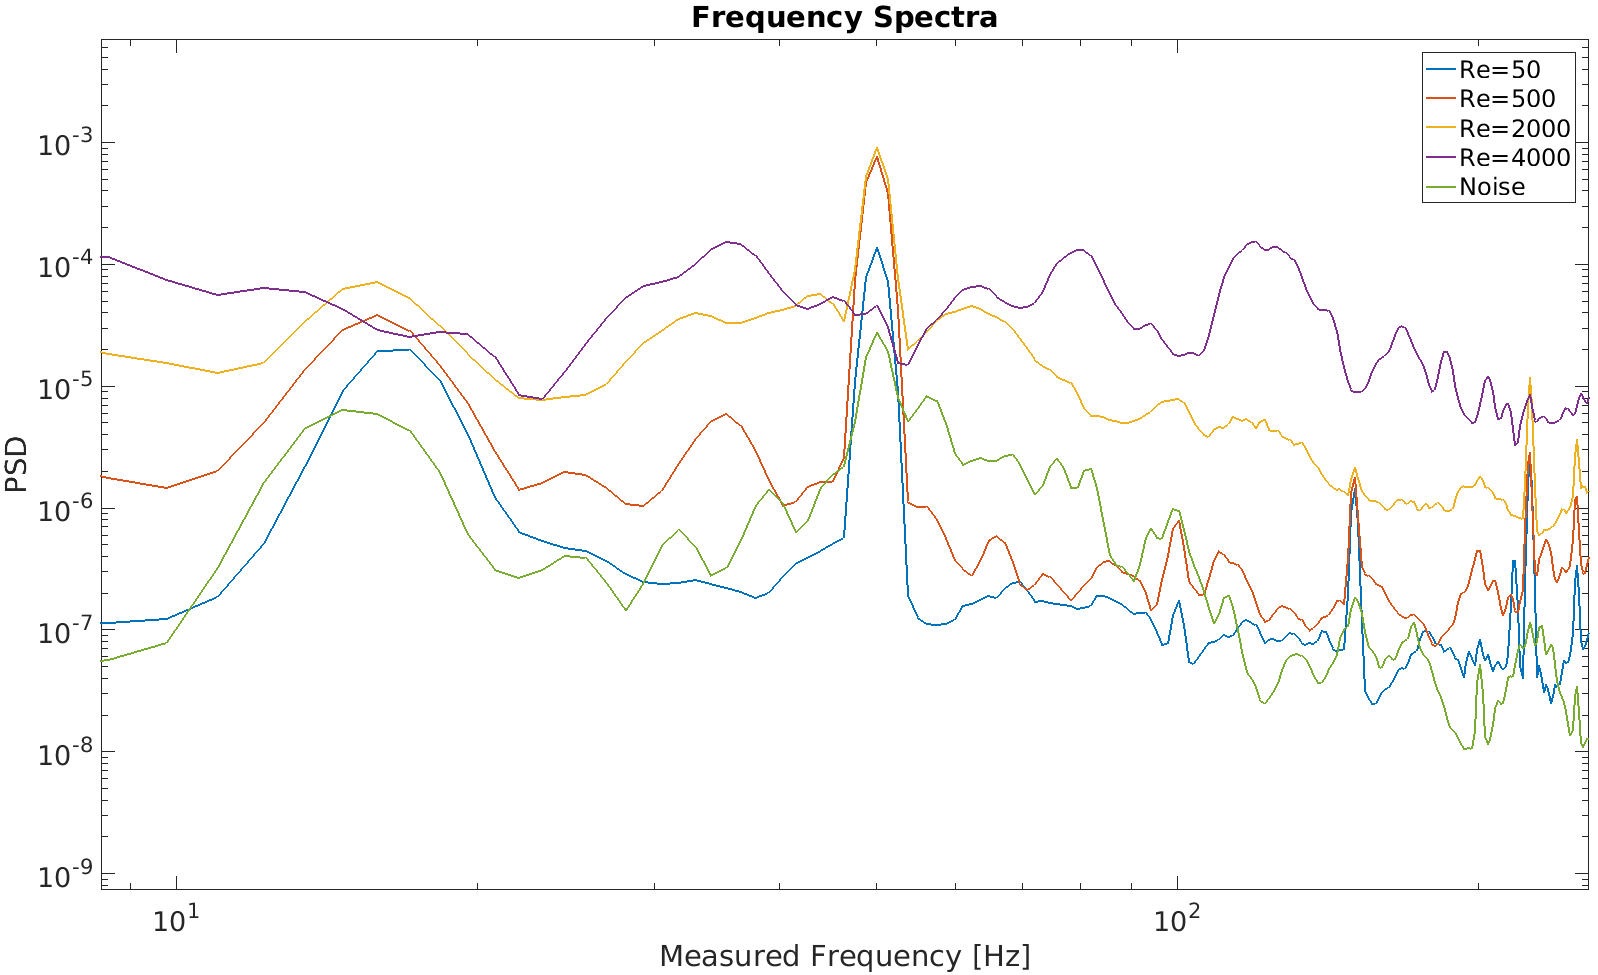
\includegraphics[width=180mm]{FrequencySpectraPlotZoomed.png}
    \caption{}
    \label{fig:4}
\end{figure}

\section*{Discussion}


\section*{Conclusion}


\section*{Appendix}
Visit the below link to see the matlab codes, the LabView files, and plots and images.

\url{https://github.com/ShakoFarhad/LabView-Project-MEK4600}

\bibliographystyle{plainnat}
\bibliography{mybib} \bigskip \bigskip
\end{document}
